\section{Results for Part I}

In this section I will show how the exact method performed under different
circumstances and describe each one of them.

\subsection{Scenarios} \label{sec:resI-scenarios}

I prepared different scenarios for the evaluation of the programs, which
correspond more or less to the different instances I provide as input with a
little of configuration.

Wrapping up, we have these different kinds of instances:

\begin{itemize}
  \item \textit{345}, i.e. the Pythagorean instance;
  \item \textit{tsp12} and \textit{tsp60}, i.e. the hard-coded instances
    provided by the professor;
  \item \textit{gerber}, i.e. an instance generated out of a Gerber file;
  \item \textit{ru}, i.e. instances generated with the Random Uniform method;s
  \item \textit{rg}, i.e. instances generated with the Random Grid Uniform
    method, in which I considered the euclidean distance between points
    ($\sqrt{(x_a - x_b)^2 + (y_a - y_b)^2}$);
  \item \textit{rg\_Manh}, i.e. instances generated with the Random Grid Uniform
    method, in which I considered the Manhattan distance between points
    ($|x_a - x_b| + |y_a - y_b|$).
\end{itemize}

While the first four instances were generated with a fixed number of
holes\footnote{I created only one Gerber instance, so I put \textit{gerber} in
the group of ``fixed'' instances}, the three random types of instances are
generated by means of some parameters:

\begin{itemize}
  \item the number of holes $n$;
  \item the size of the board $s$, which is not an absolute value but a size
    factor that, together with the number of holes, yields the actual size of
    the board\footnote{in this way, boards with different number of holes can
    be compared more reasonably};
  \item the number of divisions per side $d$ for the $rg^*$ instances, so that
    we divide the board into a grid of $d^2$ cells.
\end{itemize}

In particular, I set up the following configurations for the tests:

\begin{table}[H]
  \centering
  \begin{tabular}{|l|c|r|}
    \hline
    \textbf{\textit{h}} & \textbf{\textit{s}} & \textbf{\textit{d}} \\
    \hline
    \hline
    10 & 10  & 2 \\
    \hline
    10 & 100 & 2 \\
    \hline
    10 & 10  & 4 \\
    \hline
    10 & 100 & 4 \\
    \hline
    50 & 10  & 2 \\
    \hline
    50 & 100 & 2 \\
    \hline
    50 & 10  & 4 \\
    \hline
    50 & 100 & 4 \\
    \hline
  \end{tabular}
  \caption{Settings for tests}
  \label{tab:settings}
\end{table}

Thanks to these configurations, we range over different parameters of the
instances' creation.

\subsection{Part I performance}

Hereafter, I show how the exact method performed with each possible
configuration. For convenience, I'll group fixed-size instances together.

For each setting, at least 7 runs were executed to gather performance data.

\paragraph{Note} For these measurings, I have computed the time by looking at
the CPU cycles rather than using the wall clock time.

\paragraph{Note} Data and charts for variances will not be displayed since
variances are really small.

\paragraph{Note} Please keep in mind that the following charts displays time
performance on a \textbf{logarithmic} scale.

\begin{figure}[H]
  \centering
  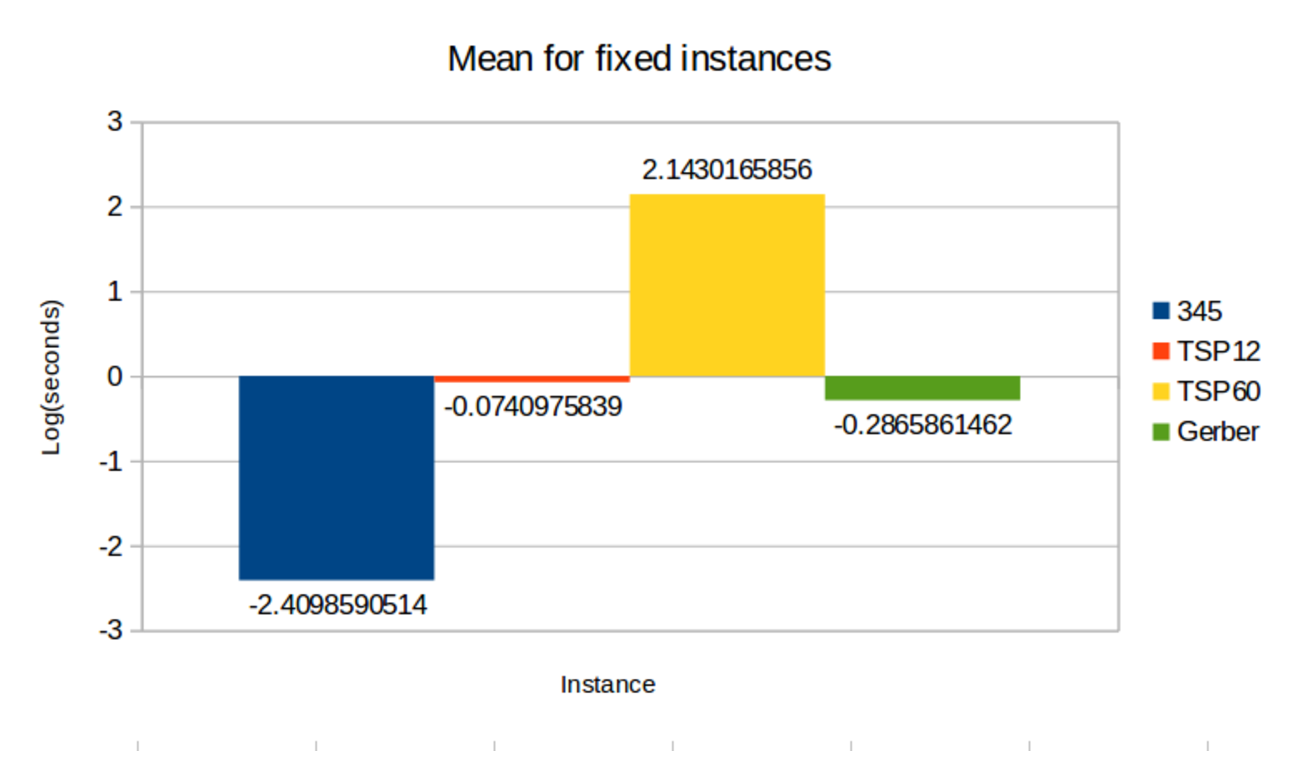
\includegraphics[width=.8\columnwidth]{pics/partI/mean-fixed.eps}
  \caption{Time performance on fixed configuration}
  \label{fig:mean-time-fixed}
\end{figure}

\begin{figure}[H]
  \centering
  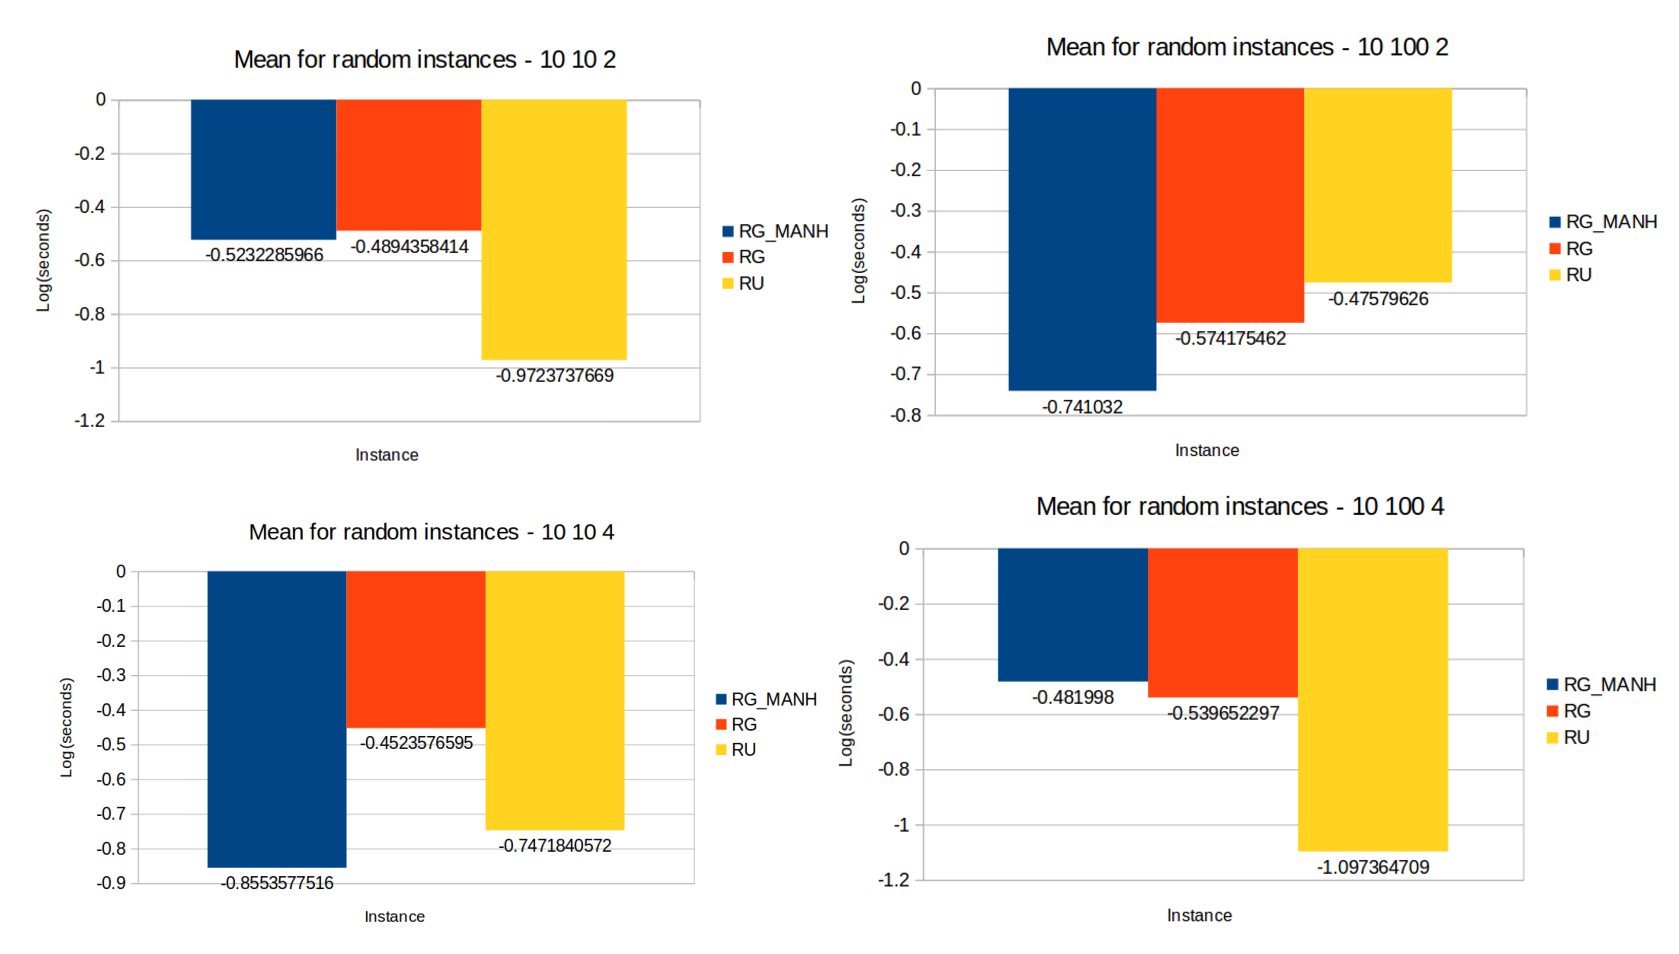
\includegraphics[width=.8\columnwidth]{pics/partI/mean-10.eps}
  \caption{Time performance on configurations with 10 holes}
  \label{fig:mean-time-10}
\end{figure}

\begin{figure}[H]
  \centering
  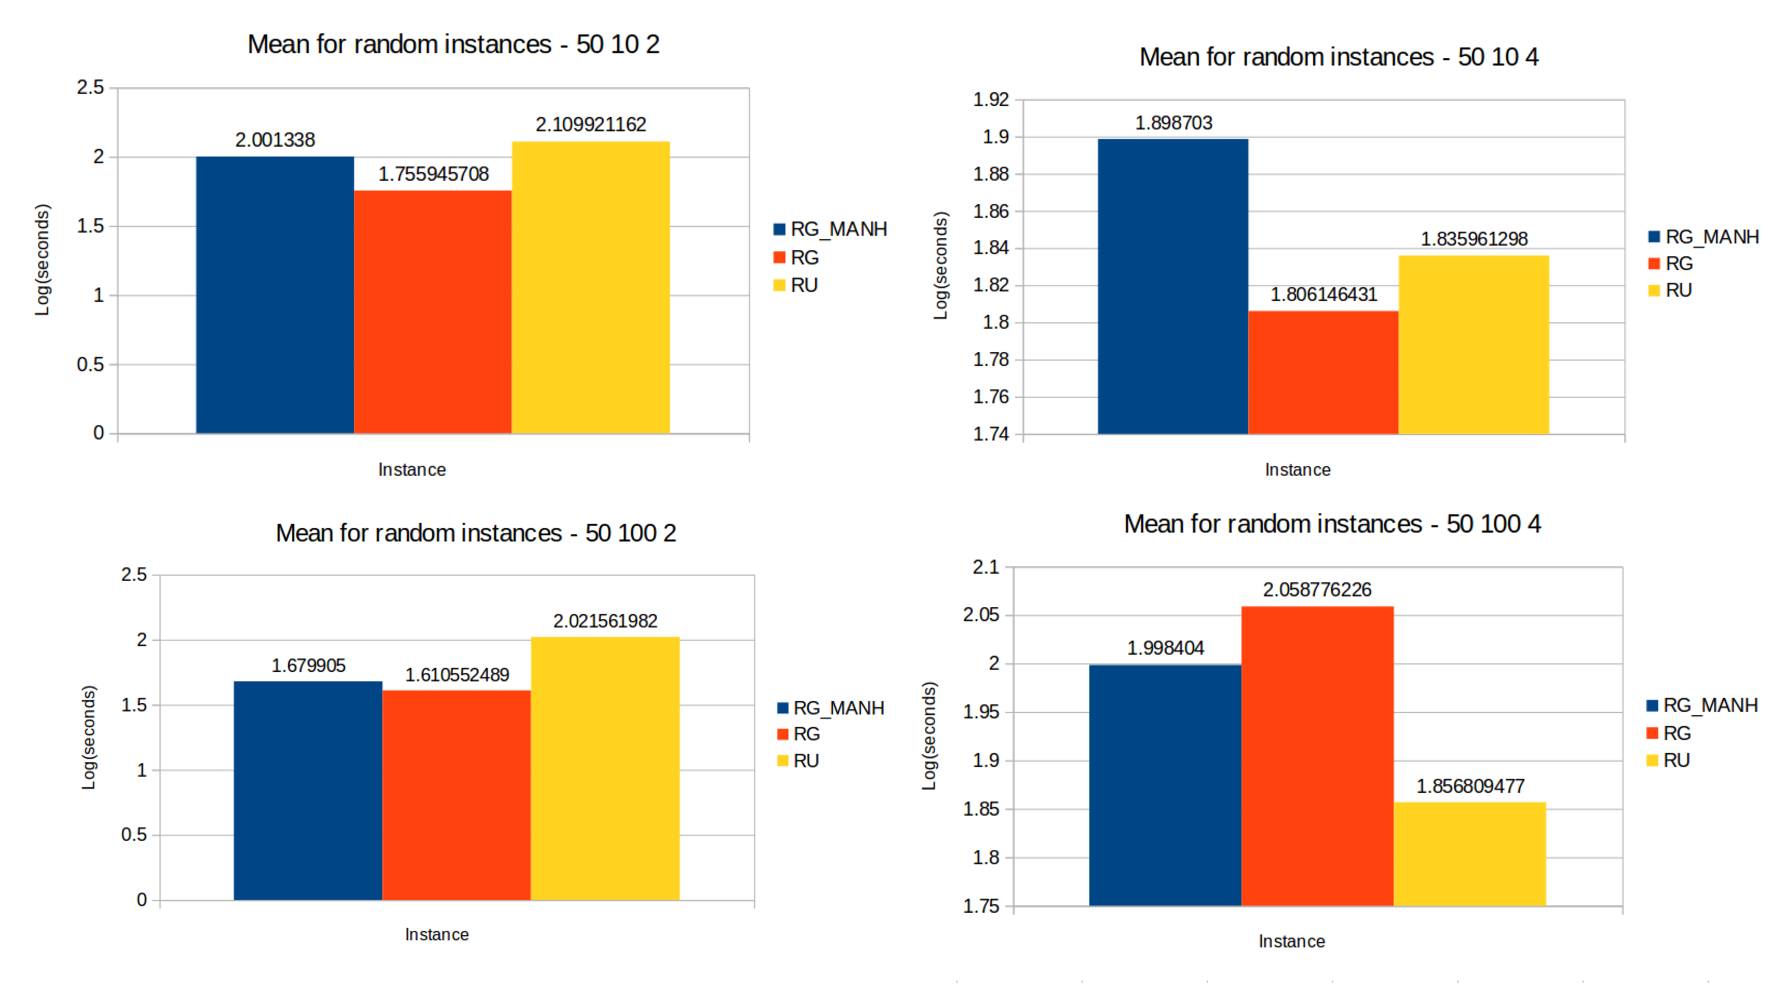
\includegraphics[width=.8\columnwidth]{pics/partI/mean-50.eps}
  \caption{Time performance on configurations with 50 holes}
  \label{fig:mean-time-50}
\end{figure}

We can understand something about these charts:

\begin{itemize}
  \item Among the fixed instances, the \textit{345} one is very easy for
    \cplex{} to solve, since it takes less than one hundredth of a second;
  \item As expected, the Gerber instance (14 holes) is more or less as
    difficult to solve as \textit{Tsp12}. However, randomly generated
    instances with 10 holes are much more easier for \cplex{} to solve since
    it took almost an order of magnitude less to find the optimal solution for
    them.
  \item The fixed instance \textit{Tsp60} is a little more demanding than the
    randomly generated ones with 50 holes, but less than a 10x factor; this
    leads me to think that when dealing with randomness sometimes we might
    incur in very tough situations (for the solver) during testing;
  \item On average, instances with Manhattan distance are easier to solve on
    boards with a few holes compared to the Random Grid instances that use the
    euclidean distance. However, this relation overturns when dealing with
    randomly generated boards that have 50 holes.
\end{itemize}
